\chapter{Conceptual study}
\label{chap:conceptual}

% \begin{toexclude}
The deciding factor for the success of one application and the failure of another is the architecture.
In order to achieve the requirements we set in the previous chapter, along with solving the issues faced by the existing solutions, we need to carefully design our systems.

In this chapter, we will first dive into the realm of real-time collaboration and read into the existing theoretical research in the field and its practical applications in the real world.
Then, we will explore the different architectures for building and scaling our application, taking into consideration our choice of collaboration algorithms.
Finally, we will present the sequence and class diagrams to better define the implementation of our ideas and the trajectory of our work in the following chapter.

\section{Real-time collaboration}

Real-time collaboration is a type of collaboration used in editors and web applications with the goal of enabling multiple users on different computers or mobile devices to modify the same document with automatic and nearly instantaneous merging of their edits.
The document could either be a computer file, stored locally, or a cloud-stored data shared over the internet, such as an online spreadsheet, a word processing document, a database, or a presentation.

Multiple web applications support real-time collaboration under various names.
Microsoft, for example, refers to it as "co-authoring" and offers it as part of its Microsoft Office bundle, including Word, Excel, and PowerPoint~\autocite{noauthor_document_nodate}.
Google Docs is another notorious contender in the space of collaborative editing, with products such as Google Docs and Google Sheets.

The interest in collaborative software has seen a resurgence since 2020, mainly due to the move to remote work, with companies like Microsoft offering ready-to-use APIs to enable this feature.

Real-time collaboration is different from other offline or delayed collaborative approaches, such as Git.
While real-time editing performs automatic, frequent, or even instantaneous synchronization of data between all the connected users, offline editing requires manual submission, merging, and resolution of editing conflicts.

\subsection{History}

In 1968, Douglas Engelbart introduced the first collaborative real-time editor in a presentation named "The Mother of All Demos", which also demonstrated many other fundamental elements of modern personal computing including windows, hypertext, graphics, video conferencing, the computer mouse, word processing, and revision control~\autocite{noauthor_firsts:_nodate}.

It took many decades for collaborative software to become mainstream.
One of the first editors that offered collaborative capabilities was Writely, a collaborative word processor launched in 2005~\autocite{chang_ehub_2005}.
It was later acquired by Google and renamed to Google Docs~\autocite{noauthor_google_2006}.
Another Google-backed product from the same era was Google Wave, a collaborative email software. However, less than a year later, it was discontinued due to a lack of users~\autocite{fried_google_nodate}.

Since 2010, the number of web-based collaborative software has been exploding with successful examples such as Figma and Notion. Figure~\ref{fig:timeline-collab} shows the resurgence of products with real-time collaboration.

\begin{figure}
  \centerfloat
  \startchronology[startyear=1960, height=0.1pc, arrow=false]
  \chronoevent{1968}{"The Mother of All Demos" \endgraf by Douglas Engelbart}
  \chronoevent[markdepth=56pt]{2006}{Writely}
  \chronoevent{2009}{Google Wave}
  \chronoevent[markdepth=104pt]{2016}{Notion}
  \chronoevent[markdepth=64pt]{2016}{Figma}
  \chronoevent[markdepth=24pt]{2018}{Notion 2}
  \stopchronology

  \caption{Timeline of real-time collaboration}
  \label{fig:timeline-collab}
\end{figure}

\subsection{Theoretical grounds}

The main challenge of real-time collaboration is keeping multiple clients in sync.
An algorithm has to be employed to determine how to apply---often conflicting---edits from the different remote users.
Network latency is the main culprit for such a dilemma as modifications can reach the other clients with a certain amount of delay.
Figure \ref{fig:collab-problem} shows a common example of conflicting changes by two users caused mainly by network latency.

\begin{figure}[H]
  \centerfloat
  \sffamily
  \begin{tikzpicture}[node distance=2.0cm]

    \node(original) {Mary};
    \node(alice-1)[below left of=original] {M\textcolor{red}{\cancel{ar}}y};
    \node(alice-2)[below of=alice-1] {My};
    \node(bob-1)[below right of=original] {\textcolor{red}{\cancel{M}}\textcolor{green}{H}ary};
    \node(bob-2)[below of=bob-1] {Hary};
    \node(result)[below right of=alice-2] {?};

    \node[right of=bob-1] {Bob};
    \node[left of=alice-1] {Alice};

    \draw[->] (original) -- (alice-1) -- (alice-2) -- (result);
    \draw[->] (original) -- (bob-1) -- (bob-2) -- (result);
  \end{tikzpicture}

  \caption{Example of a common problem in real-time collaboration}
  \label{fig:collab-problem}
\end{figure}

Over the years, two main algorithms emerged for dealing with real-time collaboration, \acrfull{crdt} and \acrfull{ot}.
Both have their benefits and drawbacks, and each one has numerous variations and implementations.

\subsubsection{\acrfull{ot}}

\acrlong{ot} was invented for supporting real-time co-editors in the late 1980s and has evolved to become a collection of core techniques widely used in today's working co-editors and adopted in major industrial products~\autocite{sun_real_2020}.
Google Docs has been using \acrshort{ot} since at least 2009~\autocite{noauthor_whats_nodate}.

The model of \acrlong{ot} works by calculating all possible transformations for a text and using them to transform received changes according to the local state, thus eliminating any possible mistakes of synchronization.
Figures~\ref{fig:ot-sol-before} and~\ref{fig:ot-sol-after} explain the algorithm followed by \acrshort{ot} for resolving conflicts.
Figure~\ref{fig:collab-sol-ot} illustrates the solution proposed by \acrshort{ot} for the problem proposed in~\ref{fig:collab-problem}.


\begin{figure}[H]
  \centerfloat
  \sffamily
  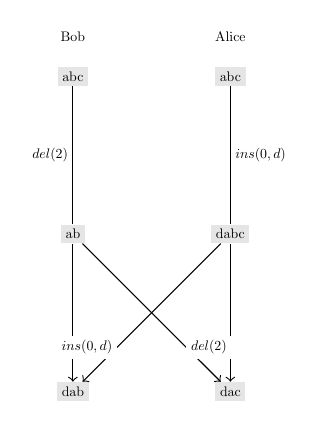
\begin{tikzpicture}[node distance=4cm,scale=0.5, every node/.append style={transform shape}]

    \node(bob-1)[rectangle, draw=none,fill=gray!20] {abc};
    \node(bob-2)[rectangle, draw=none,fill=gray!20, below of=bob-1] {ab};
    \node(bob-3)[rectangle, draw=none,fill=gray!20, below of=bob-2] {dab};

    \node(alice-1)[rectangle, draw=none,fill=gray!20, right of=bob-1] {abc};
    \node(alice-2)[rectangle, draw=none,fill=gray!20, below of=alice-1] {dabc};
    \node(alice-3)[rectangle, draw=none,fill=gray!20, right of=bob-3] {dac};

    \node at (0,1) {Bob};
    \node at (4,1) {Alice};


    \draw[->] (bob-1) --node[left]{$del(2)$} (bob-2) -- (bob-3);
    \draw[->] (alice-1) --node[right]{$ins(0,d)$} (alice-2) -- (alice-3);
    \draw[->] (alice-2) --node[left, near end,fill=white]{$ins(0,d)$} (bob-3);
    \draw[->] (bob-2) --node[right,near end,fill=white]{$del(2)$} (alice-3);
  \end{tikzpicture}
  \caption{Without \acrshort{ot}}
  \label{fig:ot-sol-before}
\end{figure}

\begin{figure}[H]
  \centerfloat
  \sffamily
  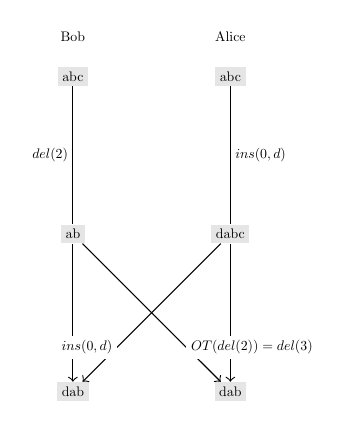
\begin{tikzpicture}[node distance=4cm,scale=0.5, every node/.append style={transform shape}]

    \node(bob-1)[rectangle, draw=none, fill=gray!20] {abc};
    \node(bob-2)[rectangle, draw=none, fill=gray!20, below of=bob-1] {ab};
    \node(bob-3)[rectangle, draw=none, fill=gray!20, below of=bob-2] {dab};

    \node(alice-1)[rectangle, draw=none, fill=gray!20, right of=bob-1] {abc};
    \node(alice-2)[rectangle, draw=none, fill=gray!20, below of=alice-1] {dabc};
    \node(alice-3)[rectangle, draw=none, fill=gray!20, right of=bob-3] {dab};

    \node at (0,1) {Bob};
    \node at (4,1) {Alice};


    \draw[->] (bob-1) --node[left]{$del(2)$} (bob-2) -- (bob-3);
    \draw[->] (alice-1) --node[right]{$ins(0,d)$} (alice-2) -- (alice-3);
    \draw[->] (alice-2) --node[left, near end,fill=white]{$ins(0,d)$} (bob-3);
    \draw[->] (bob-2) --node[right,near end,fill=white]{$OT(del(2))=del(3)$} (alice-3);
  \end{tikzpicture}
  \caption{With \acrshort{ot}}
  \label{fig:ot-sol-after}
\end{figure}


\begin{figure}[H]
  \centerfloat
  \sffamily
  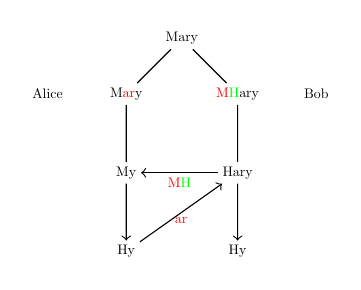
\begin{tikzpicture}[node distance=2.0cm,scale=0.5, every node/.append style={transform shape}]

    \node(original) {Mary};
    \node(alice-1)[below left of=original] {M\textcolor{red}{\cancel{ar}}y};
    \node(alice-2)[below of=alice-1] {My};
    \node(alice-3)[below of=alice-2] {Hy};
    \node(bob-1)[below right of=original] {\textcolor{red}{\cancel{M}}\textcolor{green}{H}ary};
    \node(bob-2)[below of=bob-1] {Hary};
    \node(bob-3)[below of=bob-2] {Hy};

    \node[right of=bob-1] {Bob};
    \node[left of=alice-1] {Alice};

    \draw[->] (original) -- (alice-1) -- (alice-2) -- (alice-3);
    \draw[->] (original) -- (bob-1) -- (bob-2) -- (bob-3);
    \draw[->] (bob-2) --node[below]{\textcolor{red}{\cancel{M}}\textcolor{green}{H}} (alice-2);
    \draw[->] (alice-3) --node[below]{\textcolor{red}{\cancel{ar}}} (bob-2);
  \end{tikzpicture}

  \caption{\acrshort{ot}'s solution for the problem in figure~\ref{fig:collab-problem}}
  \label{fig:collab-sol-ot}
\end{figure}

As seen in the previous examples, \acrshort{ot} can be hard and costly to set up, even for text-based documents.
When it comes to more complicated and nested data structures, \acrshort{ot} is rarely the first choice.

\subsubsection{\acrshort{crdt}}

\acrlong{crdt} is a data structure that was first proposed around 2006 under the name of \acrfull{woot}~\autocite{sun_real_2020}.
It has the benefit of being able to be duplicated over numerous computers in a network, where the replicas can be updated independently and concurrently without requiring coordination, and where inconsistencies can always be resolved mathematically~\autocite{shapiro_conflict-free_2011}.

In 2011, \acrshort{crdt} was formally defined~\autocite{shapiro_conflict-free_2011}, and while it was initially developed for collaborative text editing, it was eventually adopted for multiple other use cases such as online chat systems and distributed databases.

\acrshort{crdt} is further subdivided into two types based on its implementation---\acrfull{cmrdt} and \acrfull{cvrdt}. Both of them offer the same real-time capabilities but differ in their design and approach to the concept.

\paragraph{\acrshort{cmrdt}}

\acrlong{cmrdt} or Operation-based \acrshort{crdt} transmits the local state only by sending the update operations required to reach that state.
Upon receiving these operations, remote clients must apply them to become in sync with the sender. The transmission server has to avoid duplicating the operations as this algorithm is not idempotent.

\paragraph{\acrshort{cvrdt}}

\acrlong{cvrdt} or State-based \acrshort{crdt} sends over the whole local state to be merged with the receiving clients' states. This method tends to be slow due to the need of sending large amounts of data instantaneously over the network. However, the infrastructure does not have to deal with deduplication as it is the case with \acrshort{cmrdt}s.

\subsection{Practical examples}

In practice, web applications do not adhere to one algorithm.
Instead, they draw from different concepts to establish a solution that perfectly fits their needs.

\subsubsection{Figma}

\logofig{Figma}{figma-logo.png}

Figma is one of the first web design tools with real-time collaboration.
It was released in 2016 and since then it has been hailed as one of the best examples of performant and collaborative software~\autocite{tools_2020_nodate}.

The engineering team behind Figma avoided following the same footsteps of Google Docs in using \acrshort{ot}s, which, while performant and required less memory, were too complicated to implement and scale~\autocite{wallace_how_nodate}.
Instead, they decided to implement their real-time collaboration features using a system inspired by \acrshort{crdt}.
Since they already had a centralized server and a database acting as the source of truth, they were able to remove much of the complexity of \acrshort{crdt}s while maintaining their original concept~\autocite{wallace_how_nodate}.
In particular, the server decides which changes are applied and which ones are discarded based on the timing of these changes and their order.
This mode of operation can be viewed as a modified version of \acrshort{cmrdt}.

\lgfig{Figma collaborative interface}{figma-interface.png}{figma-interface}

\subsubsection{Excalidraw}

\logofig{Excalidraw}{excalidraw-logo.png}

Excalidraw is an open-source virtual collaborative whiteboard tool that lets you easily sketch diagrams that have a hand-drawn feel to them~\autocite{noauthor_rethinking_nodate}.
Contrary to Figma, Excalidraw is \acrfull{p2p}, that is, the server is not the source of truth and used merely for connecting the different clients and propagating changes~\autocite{noauthor_building_nodate}.
On top of that, the exchanged data is encrypted end-to-end, meaning that the server has no access to clients' changes.
Excalidraw uses a variant of \acrfull{cvrdt} with the whole state being sent over and compared to the local state before applying changes.

\lgfig{Excalidraw collaborative interface}{excalidraw-interface.jpeg}{excalidraw-interface}

What is peculiar about Excalidraw's example is the way they handle concurrent changes of the same element. Each element has a version attached to it and a hash of that version, which are compared to know which changes to apply and which ones to discard. If two clients edit the same element at the same time, Excalidraw does not try to merge those changes, instead, it picks whichever change came first~\autocite{noauthor_building_nodate}.
Figure~\ref{fig:excalidraw-algo} illustrates the algorithm implemented by Excalidraw for merging conflicting states.

\lgfig{Excalidraw collaboration algorithm as explained on their blog~\autocite{noauthor_building_nodate}}{excalidraw-algo.png}{excalidraw-algo}

\subsubsection{Automerge}

\begin{figure}[h]
  \centerfloat
  \sffamily
  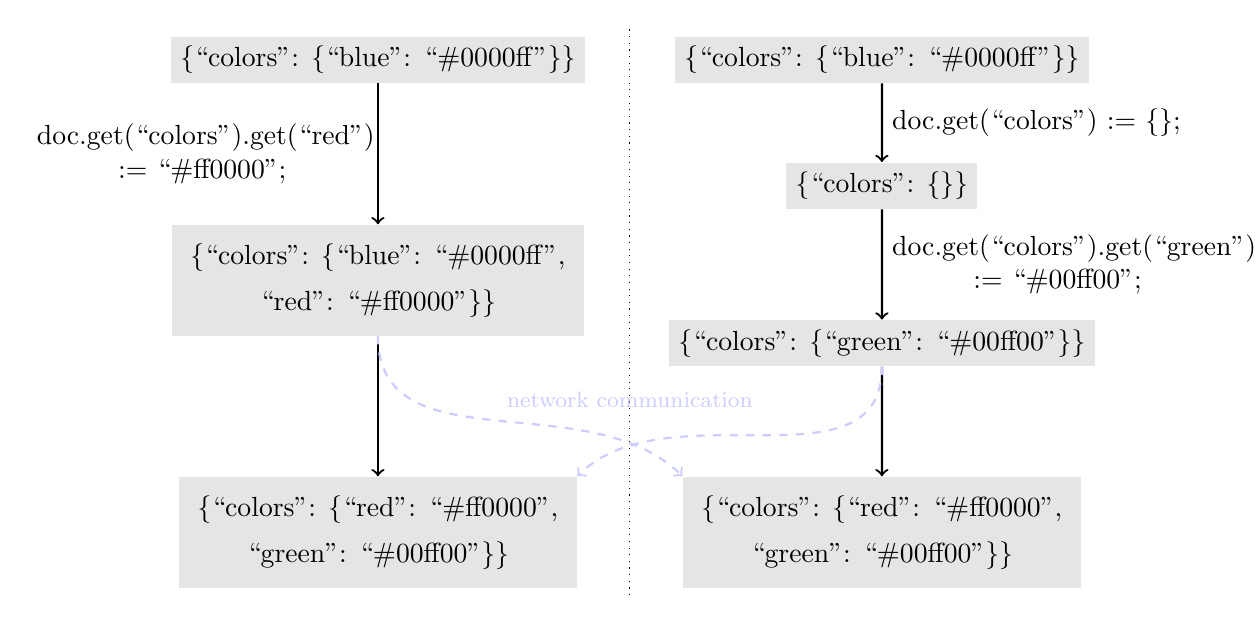
\begin{tikzpicture}[auto,scale=0.8]
    \path [draw,dotted] (4,-1) -- (4,8);
    \node (left0)  at (0,7.5) [rectangle,draw=none,fill=gray!20] {\{``colors'': \{``blue'': ``\#0000ff''\}\}};
    \node (right0) at (8,7.5) [rectangle,draw=none,fill=gray!20] {\{``colors'': \{``blue'': ``\#0000ff''\}\}};
    \node [matrix] (left1) at (0,4) [rectangle,draw=none,fill=gray!20] {
      \node {\{``colors'': \{``blue'': ``\#0000ff'',}; \\
      \node {``red'': ``\#ff0000''\}\}}; \\
    };
    \node (right1) at (8,5.5) [rectangle,draw=none,fill=gray!20] {\{``colors'': \{\}\}};
    \node (right2) at (8,3) [rectangle,draw=none,fill=gray!20] {\{``colors'': \{``green'': ``\#00ff00''\}\}};
    \node [matrix] (left2) at (0,0) [rectangle,draw=none,fill=gray!20] {
      \node {\{``colors'': \{``red'': ``\#ff0000'',}; \\
      \node {``green'': ``\#00ff00''\}\}}; \\
    };
    \node [matrix] (right3) at (8,0) [rectangle,draw=none,fill=gray!20] {
      \node {\{``colors'': \{``red'': ``\#ff0000'',}; \\
      \node {``green'': ``\#00ff00''\}\}}; \\
    };
    \node (comms) at (4,2.1) [text=blue!20] {\footnotesize network communication};
    \draw [thick,->] (left0)  -- (left1)
    node [left,text width=4.2cm,text centered,midway]  {doc.get(``colors'').get(``red'') := ``\#ff0000'';};
    \draw [thick,->] (right0) to node [right] {doc.get(``colors'') := \{\};} (right1);
    \draw [thick,->] (right1) -- (right2)
    node [right,text width=4.2cm,text centered,midway] {doc.get(``colors'').get(``green'') := ``\#00ff00'';};
    \draw [thick,->] (left1)  to (left2);
    \draw [thick,->] (right2) to (right3);
    \draw [thick,dashed,blue!20,->] (left1.south)  to [out=270,in=135] (right3.north west);
    \draw [thick,dashed,blue!20,->] (right2.south) to [out=270,in=45]  (left2.north east);
  \end{tikzpicture}
  \caption{Example of Automerge algorithms}\label{fig:automerge-algo}
\end{figure}

Automerge is a set of algorithms for applying \acrshort{crdt} concepts to a \acrfull{json} data structure without having prior knowledge of the inner working of the data structure or the infrastructure used to transmit changes.
It works by registering all the changes applied locally to the state and sending these operations to remote clients, while employing a variety of \acrshort{crdt} algorithms for resolving conflicts~\autocite{kleppmann_conflict-free_2017}. Automerge also comes with a ready-to-use JavaScript library. Figure~\ref{fig:automerge-algo} illustrates one of the algorithms provided by Automerge.

Compared to Figma, Automerge does not require any central source of truth. On top of that, it tries to resolve conflicts rather than picking one of the changes based on the version or timestamp, as it is the case in Figma and Excalidraw.

\subsubsection{Centige}

Centige is a discontinued collaborative web app builder by the author.
It was mainly a research project, started in late 2019 and developed throughout 2020, around the same time as Excalidraw.
The web application used a collaboration model very similar to that of Figma, as it relied on a centralized server acting as the source of truth and used Operation-based \acrshort{crdt} for transmitting changes to the other clients.
Each client had a \acrfull{crdt} and on ever change, the new local state would be compared with the older one, in a model similar to that of State-based \acrshort{crdt}, before generating a set of operations that are sent to the server.
The latter would compare the operations' hash before propagating them to rest of the connected clients.
All of these computations happened within milliseconds and supported offline editing to some extent.

\subsection{Our choice}

After reviewing the literature on real-time collaboration and having researched the different implementations of the feature in varying products, it is time to choose a fitting design pattern for real-time collaboration in Merebase.
It is important to keep in mind that the design of the collaborative aspect of our application greatly influences the rest of the architecture.
Considering the ease-of-use of \acrfull{crdt} and the sheer volume of the scientific literature around it, coupled with the community around it and our knowledge of the algorithm, we chose to implement a variant of \acrshort{crdt}.

In particular, we are going to implement Operation-based \acrshort{crdt} (\acrshort{cmrdt}) in approach similar to that of Excalidraw with each element having a version attached to it.
However, in contrast to Excalidraw's implementation, we are going to rely on a server a source of truth.
This choice eliminates any complexities with \acrshort{p2p} technology and keeps the performance smooth as we do not have to perform any comparisons or calculations on the client's device. Therefore, we achieve one of our non-functional requirements---speed.

\section{Architectural patterns}

To better define our technical requirements for the implementation in the upcoming chapter, it is necessary to set a list of architectural patterns to follow.
While such patterns are not set in stone, they are helpful guidelines for developing the application and avoiding any traditional pitfalls.

An architectural pattern is a general, reusable solution to a commonly occurring problem in software architecture and thus, various architectures can be mixed and used together.

\subsection{Common patterns}

As architectural patterns aim to solve various problems in different contexts, the term can be vaguely used to designate differing concepts.
% On one hand, there are patterns such as \acrfull{mvc} and \acrfull{mvvm}, which define the relation between the data and the presentation layer or the \acrfull{ui}.
% On the other hand, there are patterns such as the client-server architecture and the monolithic architecture that define the relation between the different access layers of an application.

The \acrshort{mvc} pattern, illustrated in figure~\ref{fig:mvc-arch}, tends to get paired with a monolithic architecture, illustrated in figure~\ref{fig:monolith-arch}, with a single server acting both as the data access layer and the presentation layer.
While this pattern is the most common in the software world, it is starting to fall into disuse with the proliferation of \acrshort{ui} libraries, and microservices.

\begin{figure}[H]
  \centerfloat
  \sffamily
  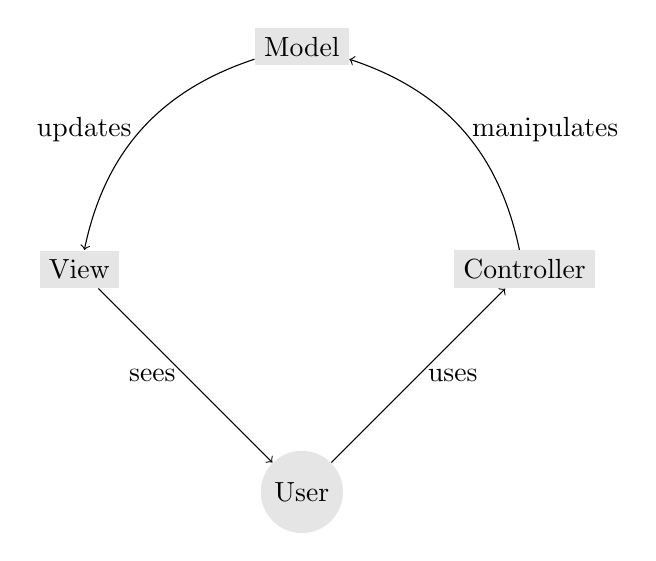
\begin{tikzpicture}[node distance=4.0cm]
    \node(model)[rectangle,fill=gray!20] {Model};
    \node(view)[rectangle,fill=gray!20, below left of=model] {View};
    \node(controller)[rectangle,fill=gray!20, below right of=model] {Controller};
    \node(user)[circle,fill=gray!20, below right of=view] {User};

    \path[->]
    (model) edge[bend right=30] node[left] {updates} (view)
    (view) edge node[left] {sees} (user)
    (controller) edge[bend right=30] node[right] {manipulates} (model)
    (user) edge node[right] {uses} (controller);
    % \draw[thick,->] (model) .. controls +(left:2cm) and +(up:2cm) .. (view);
    % \draw[thick,->] (model) .. controls +(right:2cm) and +(up:2cm) .. (controller);

  \end{tikzpicture}

  \caption{The \acrshort{mvc} pattern}
  \label{fig:mvc-arch}
\end{figure}

\begin{figure}[H]
  \centerfloat
  \sffamily
  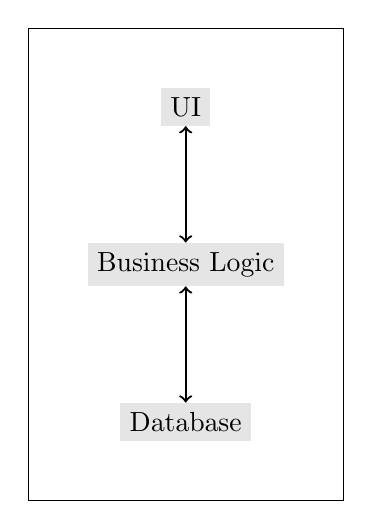
\begin{tikzpicture}
    \draw (0,0) -- (4,0) -- (4,6) -- (0,6) -- (0,0);
    \node(db)[rectangle,fill=gray!20] at (2,1) {Database};
    \node(bl)[rectangle,fill=gray!20] at (2,3) {Business Logic};
    \node(ui)[rectangle,fill=gray!20] at (2,5) {UI};

    \draw[thick, <->] (db) -- (bl);
    \draw[thick, <->] (bl) -- (ui);
  \end{tikzpicture}

  \caption{The monolith architecture}
  \label{fig:monolith-arch}
\end{figure}

More recent web applications are usually built on the \acrshort{mvvm} pattern with a modular, multitiered client-server architecture.
This focus on modularity helps in scaling and maintaining software with ease.

\subsubsection{Multitier architecture}

\begin{figure}[H]
  \centerfloat
  \sffamily
  \begin{tikzpicture}
    \draw[fill=purple!20,draw=none] (0,0)
    -- (2,0) node[midway,below] {Interface}
    -- (2,4)
    -- (0,4)
    -- (0,0);

    \draw[fill=blue!20,draw=none] (4,0)
    -- (6,0) node[midway,below] {Server}
    -- (6,4)
    -- (4,4)
    -- (4,0);

    \coordinate (x) at (9,0);

    % \draw[fill=pink!20] (8,0)
    % -- (10,0) node[midway,below] {Database}
    % -- (10,4)
    % -- (8,4)
    % -- (8,0);

    \node[cylinder,
      draw = none,
      text = black,
      cylinder uses custom fill,
      cylinder body fill = magenta!10,
      cylinder end fill = magenta!40,
      aspect = 0.2,
      % minimum size = 2cm,
      minimum height=2cm,
      minimum width=2cm,
      shape border rotate = 90, above of=x] (c) {Data};

    \path [draw,dotted] (3,-1) -- (3,5);
    \path [draw,dotted] (7,-1) -- (7,5);

    \draw[thick, <->] (2, 2) -- (4,2);
    \draw[thick, <->] (6, 2) -- (c);
  \end{tikzpicture}

  \caption{The three-tier architecture}
  \label{fig:threetier-arch}
\end{figure}

Multitier architecture or \emph{n}-tier architecture is a multilayer client-server architecture in which presentation, logic, and data are physically distinct layers. This architecture guarantees flexibility and reusability for developers since layers can be reused, removed, or expanded, without reworking the whole application.
Furthermore, it is easily scalable in case of a surge in usage or a system failure.

The most common multitier architecture is the three-tier one, illustrated in figure~\ref{fig:threetier-arch}. It is composed of:
\begin{description}
  \item[Client] It is often also called "front-end" or the interface.
        This is the tier that the end user interacts with directly.
        It is also the one where the \acrshort{mvvm} pattern is implemented.
  \item[Server] It is also called the "back-end".
        This is where the data processing and business logic happens.
  \item[Database] This is the data tier.
        It represents any system used for storing data, be it a database, or a logging storage system.
\end{description}

For more advanced use cases, it is not uncommon to see an even more distributed \emph{n}-tier architecture.
If anything, such system are quickly becoming the norm in enterprises, under the name "microservices".
In such architectures, each service is a distinct and separate tier on its own.
This architecture, however, can quickly transform from being an advantage for quick iteration and scalability to a nightmare in maintenance~\autocite{pautasso_microservices_2017}.
Therefore, each application has to find a sweet spot between scalability and flexibility, and maintainability.

\subsubsection{\acrshort{mvvm} pattern}

\begin{figure}[H]
  \centerfloat
  \sffamily
  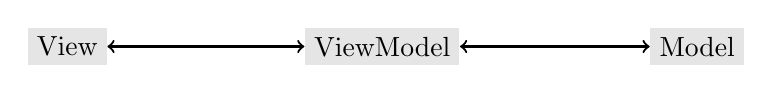
\begin{tikzpicture}[node distance=4.0cm]
    \node(m)[rectangle,draw=none, fill=gray!20] {Model};
    \node(vm)[rectangle,draw=none, fill=gray!20, left of=m] {ViewModel};
    \node(v)[rectangle,draw=none, fill=gray!20, left of=vm] {View};

    \draw[thick, <->] (v) -- (vm);
    \draw[thick, <->] (vm) -- (m);

  \end{tikzpicture}

  \caption{The \acrshort{mvvm} pattern}
  \label{fig:mvvm-arch}
\end{figure}

\acrfull{mvvm} is an architectural pattern for developing application that separates the development of the \acrfull{ui} (the \emph{view}) from the development of the backend logic (the \emph{model}) so the view is independent of the model.
The view model has the role of exposing the data of the model to the view, that is, it works as data converter.

\acrshort{mvvm} was originally a variation of the Presentation Model design pattern. It was invented in Microsoft to supported their event-driven \acrshort{ui}s, and it was incorporated into their Windows Presentation Foundation~\autocite{smith_patterns_2009}.

Most recent \acrshort{ui} frameworks, such as React, Angular, Vue.js, and Svelte, implement some variation or another of \acrshort{mvvm}~\autocite{noauthor_javascript_nodate}.

\subsection{Our choice}

Our choice of architectural patterns is largely guided by the architecture of our real-time collaboration feature and the non-functional requirements defined before, in particular speed, performance, scalability, and developer experience.

In order to achieve these goals, we can identify the following components of our architecture:

\begin{itemize}
  \item A front-end application that can stay online and functional even when the rest of the system fails;
  \item A separate view and data layers for a good developer experience;
  \item A server that can be easily scaled or replaced in case of failure or in the case of a surge in usage;
  \item Separate servers for our application and for our users' database, since an increase of demand on our application's API does not translate to an increase of demand on the application itself;
  \item A cloud-hosted database to act as the source of truth for all of our system components;
  \item An intermediate data store or pub-sub server for communicating between the different servers and keeping them in sync;
\end{itemize}

These considerations make it clear that an n-tier architecture is the most suitable for our application. Figure~\ref{fig:ntier-arch} illustrates our choice of architecture.


\begin{figure}[H]
  \centerfloat
  \tikzsetnextfilename{ntier-arch}
  \sffamily
  \begin{tikzpicture}
    \draw[fill=blue!30,draw=none] (0,0)
    -- (2,0) node[midway,below] {Interface}
    -- (2,4)
    -- (0,4)
    -- (0,0);

    \draw[fill=blue!20,draw=none] (4,-1)
    -- (6,-1) node[midway,below] {Main Server}
    -- (6,1)
    -- (4,1)
    -- (4,-1);

    \draw[fill=blue!20,draw=none] (4,3)
    -- (6,3) node[midway,below] {API Server}
    -- (6,5)
    -- (4,5)
    -- (4,3);

    \coordinate (x) at (9,-1);
    \coordinate (y) at (9,2);

    % \draw[fill=pink!20] (8,0)
    % -- (10,0) node[midway,below] {Database}
    % -- (10,4)
    % -- (8,4)
    % -- (8,0);

    \node[cylinder,
      draw = none,
      text = black,
      cylinder uses custom fill,
      cylinder body fill = purple!10,
      cylinder end fill = purple!40,
      aspect = 0.2,
      % minimum size = 2cm,
      minimum height=2cm,
      minimum width=2cm,
      shape border rotate = 90, above of=x] (c) {Database};

    \node[cylinder,
      draw = none,
      text = black,
      cylinder uses custom fill,
      cylinder body fill = red!10,
      cylinder end fill = red!40,
      aspect = 0.2,
      % minimum size = 2cm,
      minimum height=2cm,
      minimum width=2cm,
      shape border rotate = 90, above of=y] (p) {Pub-Sub};

    \path [draw,dotted] (3,-1) -- (3,5);
    \path [draw,dotted] (7,-1) -- (7,5);

    \draw[thick, <->] (2, 1) -- (4,0);
    \draw[thick, <->] (2, 3) -- (4,4);
    \draw[thick, <->] (6, 0) -- (c);
    \draw[thick, <->] (6, 0) -- (p);
    \draw[thick, <->] (6, 4) -- (c);
    \draw[thick, <->] (6, 4) -- (p);
  \end{tikzpicture}

  \caption{Our \emph{n}-tier architecture}
  \label{fig:ntier-arch}
\end{figure}

We rely on two servers to match our users' needs. The main server handles everything from business logic, data processing, and real-time collaboration, while the API server is used to compile our users' visual databases and serve them on demand in \acrshort{json} format.
This separation of concerns eliminates any system failure or scalability issues.
The Pub-Sub store is used to communicate changes between the main server(s) and the API server(s).
This is even more important when a single server could no longer match the demand, and we are required to scale our servers up.
In such cases, the Pub-Sub store would keep all of our servers in sync.


\section{Detailed architecture}

With our architectural patterns selected and our requirements fully defined, we can, now, proceed to producing detailed diagrams of our application. In the following sections, we will present our application's class, and sequence diagrams.
\subsection{Class diagrams}

Figure~\ref{fig:gen-class-diagram} represents our application's general class diagram.

\begin{figure}[hp]
  \thisfloatpagestyle{empty}
  % \centerfloat
  \centering
  \sffamily
  \tikzumlset{font=\tiny}
  \begin{tikzpicture}[scale=0.65, every node/.append style={transform shape}]
    \umlclass[x=-4,draw=none]{User}{
      ID : UUID \\
      Name : Text \\
      Email : Text \\
      Avatar : Text \\
      CreatedAt: Timestamptz \\
      ModifiedAt: Timestamptz
    }{}

    \umlclass[left=9cm of User,draw=none]{Space}{
      ID : UUID \\
      Name : Text \\
      Handle : Text \\
      CreatedAt: Timestamptz \\
      ModifiedAt: Timestamptz
    }{}


    \umlclass[below left=4cm and 1cm of Space,draw=none]{Project}{
      ID : UUID \\
      Name : Text \\
      Icon : Text \\
      Description : Text \\
      Version: Integer \\
      % SpaceID: UUID \\
      CreatedAt: Timestamptz \\
      ModifiedAt: Timestamptz
      % CreatedBy: UUID \\
      % ModifiedBy: UUID
    }{}

    % \umlclass[left=4cm of Project,draw=none]{Member}{
    %   UserID : UUID \\
    %   SpaceID : UUID \\
    %   AccessLevel: AccessLevel \\
    %   CreatedAt: Timestamptz \\
    %   ModifiedAt: Timestamptz
    % }{}

    \umlclass[right=3cm of Project,draw=none]{Confirmation}{
      % UserID : UUID \\
      % SpaceID : UUID \\
      Token: Text \\
      CreatedAt: Timestamptz \\
      ModifiedAt: Timestamptz
    }{}

    \umlclass[right=3cm of Confirmation,draw=none]{AccessToken}{
      ID : UUID \\
      Token : Text \\
      Name : Text \\
      Resource : Text \\
      ResourceID : UUID \\
      AccessLevel: AccessLevel \\
      CreatedAt: Timestamptz
      % CreatedBy: UUID
    }{}


    \umlclass[below right=2cm and 1cm of Project,draw=none]{Collection}{
      ID : UUID \\
      Name : Text \\
      Icon : Text \\
      Description : Text \\
      Version: Integer \\
      % ProjectID: UUID \\
      CreatedAt: Timestamptz \\
      ModifiedAt: Timestamptz
      % CreatedBy: UUID \\
      % ModifiedBy: UUID
    }{}

    \umlclass[below=2cm of Collection,draw=none]{Field}{
      ID : UUID \\
      Name : Text \\
      Icon : Text \\
      Description : Text \\
      Version: Integer \\
      SpaceID: UUID \\
      CreatedAt: Timestamptz \\
      ModifiedAt: Timestamptz
      % CreatedBy: UUID \\
      % ModifiedBy: UUID
    }{}

    \umlclass[right=2.5cm of Field,draw=none]{Document}{
      ID : UUID \\
      Version: Integer \\
      CollectionID: UUID \\
      CreatedAt: Timestamptz \\
      ModifiedAt: Timestamptz
      % CreatedBy: UUID \\
      % ModifiedBy: UUID
    }{}


    \umlclass[left=2.5cm of Field,draw=none]{View}{
      ID : UUID \\
      Name : Text \\
      Type : Text \\
      Data : Text \\
      Version: Integer \\
      % CollectionID: UUID \\
      CreatedAt: Timestamptz \\
      ModifiedAt: Timestamptz
    }{}

    \umlclass[below=2cm of Document,draw=none]{Block}{
      ID : UUID \\
      Data : Text \\
      % ParentID : UUID \\
      Version: Integer \\
      % FieldID: UUID \\
      % DocumentID: UUID \\
      CreatedAt: Timestamptz \\
      ModifiedAt: Timestamptz
      % CreatedBy: UUID \\
      % ModifiedBy: UUID
    }{}
    \umlclass[below=1.5cm of AccessToken, type=enumeration,draw=none]{AccessLevel}{
      Owner \\
      Admin \\
      ReadWrite \\
      ReadOnly
    }{}

    \umlnote[below=1.5cm of AccessToken, width=3cm,draw=none]{AccessToken}{
      AccessLevel is one of
      \begin{itemize}
        \item Owner
        \item Admin
        \item ReadWrite
        \item Reaonly
      \end{itemize}
    }

    \umlassoc[mult2=$1..*$,mult1=$1..*$,anchors=150 and 30]{User}{Space}

    \umlassoc[geometry=-|,mult2=$0..*$,mult1=$1$,anchors=180 and 90]{Space}{Project}

    \umlassoc[geometry=|-|,mult2=$0..*$,arg2=modifies,pos2=2.6,align2=right,mult1=$1$,anchors=130 and 100,weight=-0.35]{User}{Project}
    \umlassoc[geometry=|-|,mult2=$0..*$,arg2=creates,pos2=2.8,align2=right,mult1=$1..*$,anchors=110 and 120,weight=-0.45]{User}{Project}

    \umlassoc[geometry=|-,mult2=$0..*$,arg2=modifies,mult1=$1$,anchors=-90 and 20,pos2=1.8]{User}{Document}
    \umlassoc[geometry=|-,mult2=$0..*$,arg2=creates,mult1=$1..*$,anchors=-100 and 30,pos2=1.6]{User}{Document}

    \umlassoc[geometry=|-,mult2=$0..*$,arg2=modifies,mult1=$1$,anchors=-120 and 20,weight=0.7,pos2=1.8]{User}{Collection}
    \umlassoc[geometry=|-,mult2=$0..*$,arg2=creates,mult1=$1..*$,anchors=-130 and 30,weight=0.8,pos2=1.6]{User}{Collection}

    \umlassoc[geometry=|-,mult2=$0..*$,arg2=modifies,mult1=$1$,anchors=-60 and 20,pos2=1.8]{User}{Block}
    \umlassoc[geometry=|-,mult2=$0..*$,arg2=creates,mult1=$1..*$,anchors=-70 and 30,pos2=1.6]{User}{Block}

    \umlassoc[geometry=-|-,mult2=$0..*$,arg2=has,mult1=$1$,anchors=170 and 0,weight=0.7]{User}{Confirmation}
    \umlassoc[geometry=-|,mult2=$0..*$,arg2=has,mult1=$1$,anchors=210 and 90,weight=0.7]{User}{AccessToken}

    \umlassoc[geometry=|-|,mult2=$0..*$,arg2=has,mult1=$1$,anchors=-90 and 90]{Project}{Collection}

    \umlassoc[geometry=-|,mult2=$1..*$,arg2=has,mult1=$1$,anchors=180 and 90]{Collection}{View}
    \umlassoc[geometry=--,mult2=$1..*$,arg2=has,mult1=$1$,anchors=-90 and 90]{Collection}{Field}
    \umlassoc[geometry=-|,mult2=$1..*$,arg2=has,mult1=$1$,anchors=0 and 90]{Collection}{Document}

    \umlassoc[geometry=--,mult2=$0..*$,arg2=has,mult1=$1$,anchors=-90 and 90]{Document}{Block}
    \umlassoc[geometry=-|,mult2=$1$,arg1=has,mult1=$0..*$,anchors=180 and -90]{Block}{Field}
    \umlassoc[geometry=--,mult2=$0..*$,arg2=has,mult1=$1$,angle1=-90, angle2=0,loopsize=2cm]{Block}{Block}


  \end{tikzpicture}

  \caption{General class diagram}
  \label{fig:gen-class-diagram}
\end{figure}


\subsection{Sequence diagrams}

\begin{sdfig}{Sign up}{sign up}{sign-up}[0.6][hp][
    In order to mitigate the security issues of storing passwords, we follow the model of passwordless sign up and log in.
    Instead of asking our users for a password, which may not be as secure and unique as one might hope, we generate a \acrfull{otp} and email it to the user.
    The \acrshort{otp} is stored for a limited time in our database and it is removed once used.
    The user, therefore, has to click the confirmation link in their email in order to verify their identity.
  ]
  \umlactor[no ddots]{Visitor}
  \umlobject[no ddots,draw=none]{Interface}
  \umlobject[no ddots,draw=none]{Server}
  \umlobject[no ddots,draw=none]{Database}
  % \umlobject[no ddots,draw=none]{Pub-Sub}

  \begin{umlcall}[op={Sign up}]{Visitor}{Interface}
    \begin{umlcall}[op={Validate}]{Interface}{Interface}
      \begin{umlfragment}[type=alt, label=valid]
        \begin{umlcall}[op={Set loading}]{Interface}{Interface}
          \begin{umlcall}[op={Sign up}]{Interface}{Server}
            \begin{umlcall}[op={Has user}]{Server}{Database}
              \begin{umlfragment}[type=alt, label=true]
                \begin{umlcall}[type=return,op={Yes}]{Database}{Server}
                  \begin{umlcall}[type=return,op={Error}]{Server}{Interface}
                    \begin{umlcall}[op={Show error}]{Interface}{Interface}
                    \end{umlcall}
                  \end{umlcall}
                \end{umlcall}
                \umlfpart[else]
                \begin{umlcall}[type=return,op={No}]{Database}{Server}
                  \begin{umlcall}[op={Create user}]{Server}{Database}
                  \end{umlcall}
                  \begin{umlcall}[op={Create OTP}]{Server}{Database}
                    \begin{umlcall}[op={Send email}]{Server}{Server}
                      \begin{umlcall}[type=return,op={Ok}]{Server}{Interface}
                        \begin{umlcall}[op={Show success}]{Interface}{Interface}
                        \end{umlcall}
                      \end{umlcall}
                    \end{umlcall}
                  \end{umlcall}
                \end{umlcall}
              \end{umlfragment}
            \end{umlcall}
          \end{umlcall}
        \end{umlcall}
        \umlfpart[else]
        \begin{umlcall}[op={Show error}]{Interface}{Interface}
        \end{umlcall}
      \end{umlfragment}
    \end{umlcall}
  \end{umlcall}
\end{sdfig}

\begin{sdfig}{Log in}{log in}{log-in}
  \umlactor[no ddots]{Visitor}
  \umlobject[no ddots,draw=none]{Interface}
  \umlobject[no ddots,draw=none]{Server}
  \umlobject[no ddots,draw=none]{Database}
  % \umlobject[no ddots,draw=none]{Pub-Sub}

  \begin{umlcall}[op={Log in}]{Visitor}{Interface}
    \begin{umlcall}[op={Validate}]{Interface}{Interface}
      \begin{umlfragment}[type=alt, label=valid]
        \begin{umlcall}[op={Set loading}]{Interface}{Interface}
          \begin{umlcall}[op={Log in}]{Interface}{Server}
            \begin{umlcall}[op={Has user}]{Server}{Database}
              \begin{umlfragment}[type=alt, label=true]
                \begin{umlcall}[type=return,op={Yes}]{Database}{Server}
                  \begin{umlcall}[op={Create OTP}]{Server}{Database}
                    \begin{umlcall}[op={Send email}]{Server}{Server}
                      \begin{umlcall}[type=return,op={Ok}]{Server}{Interface}
                        \begin{umlcall}[op={Show success}]{Interface}{Interface}
                        \end{umlcall}
                      \end{umlcall}
                    \end{umlcall}
                  \end{umlcall}
                \end{umlcall}
                \umlfpart[else]
                \begin{umlcall}[type=return,op={No}]{Database}{Server}
                  \begin{umlcall}[type=return,op={Error}]{Server}{Interface}
                    \begin{umlcall}[op={Show error}]{Interface}{Interface}
                    \end{umlcall}
                  \end{umlcall}
                \end{umlcall}
              \end{umlfragment}
            \end{umlcall}
          \end{umlcall}
        \end{umlcall}
        \umlfpart[else]
        \begin{umlcall}[op={Show error}]{Interface}{Interface}
        \end{umlcall}
      \end{umlfragment}
    \end{umlcall}
  \end{umlcall}
\end{sdfig}
% \end{toexclude}


\begin{sdfig}{Confirm email}{confirm email}{confirm-email}[1][!hp][
    Upon receiving a confirmation email, the user has to click the confirm button, which sends a request to the server with the \acrshort{otp}.
    The server validates the password and either accepts it and authenticates the user, or refuses it and alarms them about the error.
    Since having users check their email every time is a poor \acrfull{ux}, the server uses time-limited browser cookies for storing the user's authentication state.
  ]
  \umlactor[no ddots]{Visitor}
  \umlobject[no ddots,draw=none]{Interface}
  \umlobject[no ddots,draw=none]{Server}
  \umlobject[no ddots,draw=none]{Database}
  % \umlobject[no ddots,draw=none]{Pub-Sub}

  \begin{umlcall}[op={Confirm}]{Visitor}{Interface}
    \begin{umlcall}[op={Confirm}]{Interface}{Server}
      \begin{umlcall}[op={Has OTP}]{Server}{Database}
        \begin{umlfragment}[type=alt, label=true]
          \begin{umlcall}[type=return,op={Yes}]{Database}{Server}
            \begin{umlcall}[op={Add cookies}]{Server}{Server}
              \begin{umlcall}[type=return,op={Ok}]{Server}{Interface}
                \begin{umlcall}[op={Redirect to home}]{Interface}{Interface}
                \end{umlcall}
              \end{umlcall}
            \end{umlcall}
          \end{umlcall}
          \umlfpart[else]
          \begin{umlcall}[type=return,op={No}]{Database}{Server}
            \begin{umlcall}[type=return,op={Error}]{Server}{Interface}
              \begin{umlcall}[op={Show error}]{Interface}{Interface}
              \end{umlcall}
            \end{umlcall}
          \end{umlcall}
        \end{umlfragment}
      \end{umlcall}
    \end{umlcall}
  \end{umlcall}
\end{sdfig}

\begin{sdfig}{Create workspace}{create workspace}{create-workspace}[1][!hp][
    Whenever a user creates a new workspace, we only ask for a name, and we intentionally create everything they may need to start working.
    This is because an empty workspace is intimidating and can slow on-boarding process for new users.
    The same process is followed whenever the user creates a project, a collection, or a document.
  ]
  \umlactor[no ddots]{Owner}
  \umlobject[no ddots,draw=none]{Interface}
  \umlobject[no ddots,draw=none]{Server}
  \umlobject[no ddots,draw=none]{Database}
  % \umlobject[no ddots,draw=none]{Pub-Sub}

  \begin{seqdigauth}[Owner]
    \begin{umlcall}[op={Create workspace}]{Owner}{Interface}
      \begin{umlcall}[op={Redirect to workspace creation}]{Interface}{Interface}
      \end{umlcall}
    \end{umlcall}
    \begin{umlcall}[op={Submit name}]{Owner}{Interface}
      \begin{umlcall}[op={Create workspace},return=Ok]{Interface}{Server}
        \begin{umlcall}[op={Create project}]{Server}{Database}
        \end{umlcall}
        \begin{umlcall}[op={Create collection}]{Server}{Database}
        \end{umlcall}
        \begin{umlcall}[op={Create field}]{Server}{Database}
        \end{umlcall}
        \begin{umlcall}[op={Create view}]{Server}{Database}
        \end{umlcall}
        \begin{umlcall}[op={Create document}]{Server}{Database}
        \end{umlcall}
        \begin{umlcall}[op={Create block}]{Server}{Database}
        \end{umlcall}
      \end{umlcall}
    \end{umlcall}
  \end{seqdigauth}
\end{sdfig}

% \begin{toexclude}

\begin{sdfig}{Create collection}{create collection}{create-collection}[1][!hp]
  \umlactor[no ddots]{Editor}
  \umlobject[no ddots,draw=none]{Interface}
  \umlobject[no ddots,draw=none]{Server}
  \umlobject[no ddots,draw=none]{Database}
  % \umlobject[no ddots,draw=none]{Pub-Sub}

  \begin{seqdigauth}[Editor]
    \begin{umlcall}[op={Create collection},return=Ok]{Editor}{Interface}
      \begin{umlcall}[op={Create collection},return=Ok]{Interface}{Server}
        \begin{umlcall}[op={Create collection}]{Server}{Database}
        \end{umlcall}
        \begin{umlcall}[op={Create field}]{Server}{Database}
        \end{umlcall}
        \begin{umlcall}[op={Create view}]{Server}{Database}
        \end{umlcall}
        \begin{umlcall}[op={Create document}]{Server}{Database}
        \end{umlcall}
        \begin{umlcall}[op={Create block}]{Server}{Database}
        \end{umlcall}
      \end{umlcall}
    \end{umlcall}
  \end{seqdigauth}
\end{sdfig}


\begin{sdfig}{Create field}{create field}{create-field}[1][!hp]
  \umlactor[no ddots]{Editor}
  \umlobject[no ddots,draw=none]{Interface}
  \umlobject[no ddots,draw=none]{Server}
  \umlobject[no ddots,draw=none]{Database}
  % \umlobject[no ddots,draw=none]{Pub-Sub}

  \begin{seqdigauth}[Editor]
    \begin{umlcall}[op={Create field}]{Editor}{Interface}
    \end{umlcall}

    \begin{umlcall}[op={Select type},return=Ok]{Editor}{Interface}
      \begin{umlcall}[op={Update local state}]{Interface}{Interface}
      \end{umlcall}
      \begin{umlcall}[op={Create field},return=Ok]{Interface}{Server}
        \begin{umlcall}[op={Create field}]{Server}{Database}
        \end{umlcall}
        \begin{umlcall}[op={Create blocks}]{Server}{Database}
        \end{umlcall}
      \end{umlcall}
    \end{umlcall}
  \end{seqdigauth}
\end{sdfig}

\begin{sdfig}{Update block}{update block}{update-block}[0.7][!hp][
    Updating a block is the most common task in our application. It happens within milliseconds and it is quickly propagated to all the connected collaborators.
    This work by first updating the local state in order to give the effect of an immediate change. Then, the updated block is sent to the server, which would compare its version with the one stored in the database---our source of truth.
    The equality of versions means that the user has an up-to-date local state, and therefore, their change is accepted and sent to the other users. However, the unequality of versions indicates that the user's local state is out-of-date. Since they are online, they will eventually get the missing updates. So, their change is refused.
    The same method applies to updating fields too.
  ]
  \umlactor[no ddots]{Editor}
  \umlobject[no ddots,draw=none]{Interface}
  \umlobject[no ddots,draw=none]{Server}
  \umlobject[no ddots,draw=none]{Database}
  \umlobject[no ddots,draw=none]{Pub-Sub}

  \begin{seqdigauth}[Editor]
    \begin{umlcall}[op={Update block}]{Editor}{Interface}
      \begin{umlcall}[op={Update local state}]{Interface}{Interface}
      \end{umlcall}
      \begin{umlcall}[op={Update block}]{Interface}{Server}
        \begin{umlcall}[op={Get block}]{Server}{Database}
        \end{umlcall}

        \begin{umlcall}[op={Compare versions}]{Server}{Server}
          \begin{umlfragment}[type=alt, label=equal]
            \begin{umlcall}[op={Update block}]{Server}{Database}
            \end{umlcall}
            \begin{umlcall}[op={Propagate change}]{Server}{Pub-Sub}
            \end{umlcall}
            \begin{umlcall}[op={Propagate}]{Pub-Sub}{Pub-Sub}
            \end{umlcall}
            \umlfpart[else]
            \begin{umlcall}[op={Refuse change},type=return]{Server}{Interface}
              \begin{umlcall}[op={Update local state}]{Interface}{Interface}
              \end{umlcall}
            \end{umlcall}
          \end{umlfragment}
        \end{umlcall}
      \end{umlcall}
    \end{umlcall}
  \end{seqdigauth}
\end{sdfig}

% \subsection{Activity diagrams}
\section{Conclusion}

In this chapter, we analyzed the possible architectures of the different aspects of our applications, compared them, and made an objective choice.
Then, we proceeded to present, in details, the architecture of our application.

Within the next chapter, we are going to glue all the pieces of research and theory together, and bring our application to life.

% \end{toexclude}
